\chapter{Differential Algebraic Equations}

von \cite{NumerikGewöhnlicherDifferentialgleichungen} und DAE lecture

The resulting MNA of electrical circuits leads to a special form of differential equations, namely \emph{differential algebraic equations} (DAE). Additionally to differential equations they also contain algebraic equations or are equivalent to such a system. They are distinct from ordinary differential equations in that the Jacobian matrix for a DAE system is singular. 
To understand the general solvability of those systems and to find good numerical methods we first have to take a look at the theory of such DAEs.

In the most general form a DAE can be written as:
Find $y:\mathbb{R} \to \mathbb{R}^n$ such that
\begin{equation}
	\label{Abstract_DAE}
	F(t, y(t), y'(t)) = 0, \qquad \forall t \in I
\end{equation}

with $F:\mathbb{R} \times \mathbb{R}^n \times \mathbb{R}^n \to \mathbb{R}^n$ sufficiently smooth and $I$ the time-interval. As this is usually too general, one has to consider more specific types of DAEs.
This chapter focuses on giving a brief overview of the different types of differential algebraic equations. We will discuss the specific form of linear systems with constant coefficients in more detail, as those are the systems that arise from modified nodal analysis of a RLC-system. Additionally this chapter also discusses the notion of the index of an MNA-system.

\section{Types of DAEs}

	Commonly systems of either of the three types below are considered when talking about DAEs.
	
	\begin{itemize}
		\item \textbf{Linear systems with constant coeffiecients} \newline
		are systems of the form: find $y$ such that
		\begin{equation}
			\label{DAE-const-coeff}
			A y'(t) + B y(t) = f(t) ,
		\end{equation}
		with $A,B \in \mathbb{R}^{n \times n}$, $A$ singular, $B$ regular and $f:\mathbb{R} \to \mathbb{R}^n$ a function in time. If $A$ is regular this equation can be transformed into an ordinary differental equation, since
		\begin{displaymath}
			y'(t) + A^{-1}By(t) = A^{-1} f(t)
		\end{displaymath}
		
		Thus it is reasonable to assume $A$ singular.
		
		\item \textbf{Linear time dependent systems}
		are systems of the form: find $y$ such that
		\begin{displaymath}
			A(t) y'(t) + B(t) y(t) = f(t) ,
		\end{displaymath}
		with $A, B:\mathbb{R} \to \mathbb{R}^{n \times n}$, $f:\mathbb{R} \to \mathbb{R}^n$ functions, such that for every $t \in \mathbb{R}$ the matrix $A(t)$ is singular and the matrix $B(t)$ regular.
		
		\item  \textbf{Structured (non-linear) systems} \newline
		are semi-explicit systems of the form: find $(y,z)$ such that
		\begin{align}
			y'(t) &= f(t, y(t), z(t)) , \\
			0 &= g(t,y(t),z(t)) ,
		\end{align}
		with $f:\mathbb{R} \to \mathbb{R}^n$ and $g:\mathbb{R} \to \mathbb{R}^d$ functions.
	\end{itemize}
	
	For our analysis of electrical networks we will focus on linear systems with constant coefficients. The other systems could for example occur when we also consider time-dependant component relations e.g. Temperature.

\subsection{Weierstraß-Kronecker Normalform}
\label{chap:Weierstraß-Kronecker Normalform}
%kapitel aus buch seite 399 num gew dgl steif, kapitel 13.2.2

To determine the solvability of a linear system with constant coefficients \eqref{DAE-const-coeff} we first need to introduce a normalform for the system, the \emph{Weierstraß-Kronecker normalform}. This normalform is dependent on the family $\{A,B\} := \{ \mu A+B|\mu \in \mathbb{R} \}$, which is called the  \emph{matrix pencil} of the DAE.

\begin{definition}
	The matrix pencil $\{ A,B\}$ is called \emph{regular} if there exists some $c \in \mathbb{R}$, such that $(cA+B)$ is regular (i.e. $det(cA+B) \neq 0$), otherwise it is called singular.
\end{definition}

\begin{theorem}[Jordan Normalform \protect{\cite[Theorem~13.2.1]{NumerikGewöhnlicherDifferentialgleichungen}}]
	For every matrix $Q \in \mathbb{R}^{n \times n}$ there exists a regular matrix $T \in \mathbb{C}^{n \times n}$, such that
	\begin{displaymath}
		T^{-1}QT = J = diag(J_1, ..., J_r) \quad \text{with} \quad J_i = 
		\left(
		\begin{matrix}
			\lambda_i & 1 & & 0 \\
			0 & \lambda_i & \ddots & \vdots \\
			& \ddots & \ddots & 1 \\
			0 & \hdots & 0 & \lambda_i
		\end{matrix}
		\right)
		\in \mathbb{C}^{m_i \times m_i}
	\end{displaymath} 
	and $n = m_1 + ... + m_r$.
\end{theorem}

The matrix $J$ is called Jordan Normalform of $Q$, the matrices $J_i$ are called Jordan Blocks, where $\lambda_i$ are corresponding the eigenvalues of $Q$. The matrix $J$ is uniquely determined by $Q$ except for the arrangement of the diagonal blocks. If $Q$ posesses only real eigenvalues, then $T$ can also be choosen from the reals. \newline
A transformation from $A$ and $B$ in \ref{DAE-const-coeff} enables a seperation into differential and algebraic variables.	
%aus buch seite 401
\begin{theorem}[\protect{\cite[Satz~13.2.2]{NumerikGewöhnlicherDifferentialgleichungen}}]
	\label{Kronecker-Normalform}
	Let $\{ A,B \}$ be a regular matrix pencil. There exist $P,Q \in \mathbb{C}^{n \times n}$ such that
	\begin{displaymath}
		PAQ = 
		\left(
		\begin{matrix}
			I_d & 0 \\
			0 & N 
		\end{matrix}
		\right), \quad
		PBQ = 
		\left(
		\begin{matrix}
			R & 0 \\
			0 & I_{n-d}
		\end{matrix}
		\right)
	\end{displaymath}

	where
	\begin{displaymath}
		N = diag(N_1, ..., N_r) \quad \text{with} \quad N_i = 
		\left(
		\begin{matrix}
			0 & 1 & & 0\\
			& \ddots &\ddots & \\
			& & & 0 & 1 \\
			0 & & & 0
		\end{matrix}
		\right)
		\in \mathbb{R}^{n_i \times n_i}
	\end{displaymath}
	and R has Jordan Normalform. By $I_k$ we denote the identity matrix of size $k \times k$.
\end{theorem}

\begin{proof}
	Because $\{A,B\}$ is a regular matrix pencil, there exists $c \in \mathbb{R}$ such that $(cA+B)$ is regular. Set
	\begin{displaymath}
		\hat{A} := (cA+B)^{-1}A, \quad \hat{B} := (cA+B)^{-1}B.
	\end{displaymath}
	Considering 
	\begin{displaymath}
		(cA+B)^{-1}(cA+B) = I \implies (cA+B)^{-1}B+c(cA+B)^{-1}A = I ,
	\end{displaymath}
	we get that
	\begin{displaymath}
		\hat{B} = I-c \hat{A} .
	\end{displaymath}
	Let $J_ {\hat{A}}$ be the Jordan Normalform of $\hat{A}$, this means that there exists a regular matrix $T_1$ such that
	\begin{displaymath}
		T_1^{-1}AT_1 = J_{\hat{A}} =
		\left(
		\begin{matrix}
			W & 0 \\
			0 & \tilde{N} 
		\end{matrix}
		\right) .
	\end{displaymath}
	The matrix $W$ contains the Jordanblocks with Eigenvalues which are nonzero, the matrix $\tilde{N}$ contains the Jordan blocks with Eigenvalues equal to zero, thus $\tilde{N}$ is \emph{nilpotent}.
	The Jordan Normalform $J_{\hat{B}}$ of $\hat{B}$ is given by
	\begin{displaymath}
		T_1^{-1} \hat{B} T_1 = J_{\hat{B}} = 
		\left(
		\begin{matrix}
			I-cW & 0 \\
			0 & I-c\tilde{N}
		\end{matrix}
		\right) .
	\end{displaymath}
	The following two transformations will allow us to get the desired structure.
	First we will transform $J_{\hat{A}}$ with
	\begin{displaymath}
		T_2 :=
		\left(
		\begin{matrix}
			W & 0 \\
			0 & I-c\tilde{N}
		\end{matrix}
		\right)
	\end{displaymath}
	in
	\begin{displaymath}
		T_2^{-1}J_{\hat{A}} = 
		\left(
		\begin{matrix}
			I & 0 \\
			0 & (I-c\tilde{N})^{-1}\tilde{N}
		\end{matrix}
		\right)
	\end{displaymath}
	and $J_{\hat{B}}$ in
	\begin{displaymath}
		T_2^{-1}J_{\hat{B}} =
		\left(
		\begin{matrix}
			W^{-1}-cI & 0 \\
			0 & I
		\end{matrix}
		\right) .
	\end{displaymath}
	Let now $R$ be the Jordan Normalform of $(W^{-1}-cI)$ and $N$ be the Normalform of $(I-c\tilde{N})^{-1}\tilde{N}$, this means
	\begin{displaymath}
		T_W^{-1}(W^{-1}-cI)T_W = R \quad \text{and} \quad T_{\tilde{N}}^{-1}(I-c\tilde{N})^{-1}\tilde{N}T_{\tilde{N}} = N
	\end{displaymath}

	Considering this definition together with the Neumann-series of $(I-c\tilde{N})^{-1}$ we obtain
	\begin{displaymath}
		\tilde{N} (I-c\tilde{N})^{-1} = \tilde{N} (c \sum_{i=0}^{\infty} \tilde{N}^i) = \tilde{N} (c \sum_{i=0}^{k-1} \tilde{N}^i) = c \sum_{i=0}^{k-1} \tilde{N}^{i+1} = (c \sum_{i=0}^{k-1} \tilde{N}^{i}) \tilde{N}
	\end{displaymath}
	where we used that $\tilde{N}$ is nilpotent with nilpotency index $k$. This shows that $\tilde{N}$ and $(I-c\tilde{N})^{-1}$ commute.
	
	From this we can conclude that
	\begin{displaymath}
		N^k = [T_{\tilde{N}}^{-1}(I-c\tilde{N})^{-1}\tilde{N}T_{\tilde{N}}]^k = T_{\tilde{N}}^{-1}[(I-c\tilde{N})^{-1}\tilde{N}]^kT_{\tilde{N}} = T_{\tilde{N}}^{-1}(I-c\tilde{N})^{-k}\underbrace{\tilde{N}^k}_{=0}T_{\tilde{N}} = 0
	\end{displaymath}
	
	We used the commutativity in the third step here. The nilpotent matrix $N$ thus also has the nilpotency index $k$. A transformation with
	\begin{displaymath}
		T_3 := 
		\left(
		\begin{matrix}
			T_W & 0 \\
			0 & T_{\tilde{N}}
		\end{matrix}
		\right)
	\end{displaymath}
	transforms $T_2^{-1}J_{\hat{A}}$ into the Jordan Normalform
	\begin{displaymath}
		J_{\tilde{A}} := T_3^{-1}T_2^{-1}J_{\hat{A}}T_3 = T_3^{-1}T_2^{-1}T_1^{-1}\hat{A}T_1T_3 = 
		\left(
		\begin{matrix}
			I & 0 \\
			0 & N
		\end{matrix}
		\right)
	\end{displaymath}
	and $T_2^{-1}J_{\hat{B}}$ into
	\begin{displaymath}
		J_{\tilde{B}} := T_3^{-1}T_2^{-1}J_{\hat{B}}T_3 = T_3^{-1}T_2^{-1}T_1^{-1}\hat{B}T_1T_3 = 
		\left(
		\begin{matrix}
			R & 0 \\
			0 & I
		\end{matrix}
		\right) .
	\end{displaymath}
	Now set
	\begin{displaymath}
		P:= T_3^{-1}T_2^{-1}T_1^{-1}(cA+B)^{-1} \quad \text{and} \quad Q = T_1T_3
	\end{displaymath}
	to get the statement.
\end{proof}

Using the findings above we are able to transform the initial DAE \eqref{DAE-const-coeff} using the matrix $P$ from Theorem \ref{Kronecker-Normalform}. By multiplying with $P$ from the left, we obtain
\begin{displaymath}
	P A y'(t) + P B y(t) = P f(t) .
\end{displaymath}

Setting
\begin{displaymath}
	y(t) = Q
	\left(
	\begin{matrix}
		u(t) \\
		v(t)
	\end{matrix}  
	\right) 
	, \quad
	Pf(t) = 
	\left(
	\begin{matrix}
		s(t) \\
		q(t)
	\end{matrix}
	\right)
	\quad \text{with} \quad
	u(t),s(t) : \mathbb{R} \to \mathbb{R}^d ,
\end{displaymath}

we get a system of the form
\begin{equation}
	\label{transformed-DAE-const-coeff}
	\begin{aligned}
		u'(t) + Ru(t) &= s(t), \\
		Nv'(t) + v(t) &= q(t).
	\end{aligned}
\end{equation}

Where $PAQ = 
\left( 
\begin{matrix}
	I & \\
	 & N
\end{matrix} 
\right)$
and $PBQ = 
\left( 
\begin{matrix}
	R & \\
	 & I
\end{matrix} 
\right)$.

We call this system the\emph{ Weierstraß-Kronecker normalform} of the DAE. The first equation of \eqref{transformed-DAE-const-coeff} is a first order ordinary differential equation and posesses a unique solution $u(t)$ in $[t_0,t_l]$ for any initial values $u_0 \in \mathbb{R}^d$. Now let $q(t) \in C^{k-1}([t_0,t_l])$, where $C^{k-1}(I)$ denotes the space of all functions with domain $I$ that are $k-1$ times differentiable. We differentiate the second equation in \eqref{transformed-DAE-const-coeff} and obtain
\begin{align}
	\notag
	v(t) &= q(t) - Nv'(t) = q(t) - N(\underbrace{q(t)-Nv'(t)}_{=v(t)})' = q-Nq'+N^2v'' \\ \notag
	&= q-Nq'+N^2(q-Nv')'' = q-Nq'+N^2q''-N^3v''' \\ \notag
	&\vdots \\ \notag
	&= q-Nq'+...+(-1)^{k-1}N^{k-1}\underbrace{\frac{d^k}{dt^k}q}_{:=q^{(k-1)}}+(-1) \underbrace{N^kv^{(k)}}_{=0}\\ 
	\label{solution-to-transformed-DAE-const-coeff-part2}
	&= \sum_{i=0}^{k-1} (-1)^iN^iq^{(i)}(t)
\end{align}

where $k$ is the nilpotency index of $N$. Hence we have an explicit  form of the solution of $v(t)$. The Kronecker index $k$ thus tells us how many differentiations are required to obtain an ordinary differential equation.

We can also give a general definition of a DAE in Weierstraß-Kronecker normalform.
\begin{definition}[\protecting{\cite[Definition~13.2.4]{NumerikGewöhnlicherDifferentialgleichungen}}]
	A linear differential equation \eqref{DAE-const-coeff} is said to be in Weierstraß-Kronecker normalform if
	\begin{displaymath}
		A = 
		\left(
		\begin{matrix}
			I & 0 \\
			0 & N
		\end{matrix}
		\right), \quad
		B = 
		\left(
		\begin{matrix}
			R & 0 \\
			0 & I
		\end{matrix}
		\right),
	\end{displaymath}
	where $N$ is a nilpotent Jordan-block matrix.
\end{definition}

\begin{definition}
	The nilpotency index $k$ of the matrix $N$ from the Weierstraß-Kronecker Normalform of a matrix pencil $\{A,B\}$ with $A$ singular is called the \emph{Kronecker-Index} of $\{A,B\}$, which we denote by $ind\{A,B\}$. Note that for $A$ regular we set $ind\{A,B\} = 0$.
\end{definition}

%lemma 13.2.1

\begin{lemma}
	\label{Lemma:indipendence of Kronecker index}
	The Kronecker-Index $ind\{A,B\}$ is independant of the choice of the matrices $P$ and $Q$.
\end{lemma}

\begin{proof}
	See ... in \protect{\cite[\pno403]{NumerikGewöhnlicherDifferentialgleichungen}}.
\end{proof}

%\begin{figure}
%	\centering
%	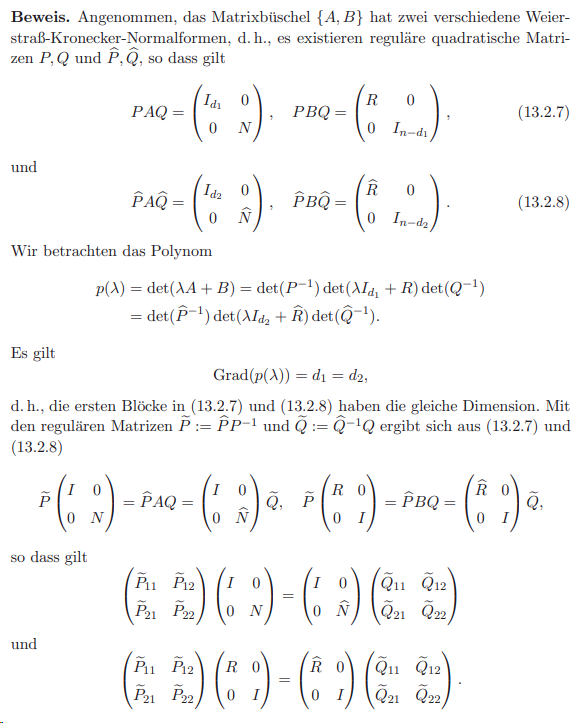
\includegraphics[width=0.7\linewidth]{screenshot003}
%	\caption{}
%	\label{fig:screenshot003}
%\end{figure}

%\begin{figure}
%	\centering
%	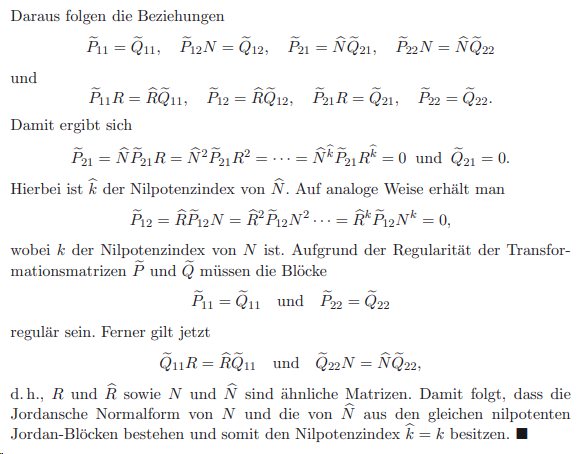
\includegraphics[width=0.7\linewidth]{screenshot004}
%	\caption{}
%	\label{fig:screenshot004}
%\end{figure}


%Lemma 13.2.2



\section{Index of a Differential Algebraic Equation}

The index of a DAE gives us insight about its numerical properties and in general about the solvability where the intuition is ``The higher the index, the harder to solve''.

We will consider two types of index concepts, the differentiation index and the perturbation index.

Since numerical differentiation is an unstable procedure the differentiation index aims to give a measure for the numerical problems to be expected when solving such systems.

\begin{definition}[differentiation index \protect{\cite[Definition~13.3.1]{NumerikGewöhnlicherDifferentialgleichungen}}]
	Consider the differential algebraic equation \eqref{Abstract_DAE} to be uniquely locally solvable and $F$ sufficiently smooth. For a given $m \in \mathbb{N}$ consider the equations
	\begin{displaymath}
		\begin{aligned}
			F(t,y,y') &= 0, \\
			\diff{F(t,y,y')}{t} &= 0, \\
			&\vdotswithin{=} \\
			\diff[m]{F(t,y,y')}{t} &= 0.
		\end{aligned}
	\end{displaymath}
	The smallest natural number $m$ for which the above system results in an explicit system of ordinary differential equations (ODEs), i.e. it has the form
	\begin{displaymath}
		y' = \phi(t,y),
	\end{displaymath}
	is called \textbf{differentiation index}.
\end{definition}

In the previous chapter we have already discussed, that for a DAE with constant coefficients \eqref{DAE-const-coeff} and a regular matrix pencil $\{A,B\}$  we need $k = ind\{A,B\}$ differentiations to receive an ordinary differential equation. Hence for a DAE with constant coefficients the Kronecker index $k$ is equal to the differentiation index.

\begin{definition}[perturbation index \protect{\cite[Definition~13.3.3]{NumerikGewöhnlicherDifferentialgleichungen}}]
	Let $y(t)$ be the exact solution of \eqref{Abstract_DAE} and $\tilde{y}(t)$ be the solution of the perturbed system $F(t, \tilde{y}, \tilde{y}') = \delta(t)$. The smallest number $k \in \mathbb{N}$ such that 
	\begin{displaymath}
		||y(t)-\tilde{y}(t)|| \leq C \left(||y(t_0)-\tilde{y}(t_0)||+\sum_{j=0}^{k}\max_{t_0 \leq \xi \leq T} \left\rVert 		\int_{t_0}^{\xi}\diff[j]{\delta}{\tau}(\tau)d \tau \right\rVert \right)
	\end{displaymath}
	for all $\tilde{y}(t)$, is called the \textbf{perturbation index} of this system.
\end{definition}	

In the case of linear DAEs with constant coefficients and a regular matrix pencil $\{A,B\}$, we can transform the DAE
\begin{displaymath}
	A(y'(t)-\tilde{y}'(t)) + B(y'(t)-\tilde{y}(t)) = \delta(t)
\end{displaymath}

into% (\textbf{how?} - bemerkung 13.3.5
\begin{align*}
	u'(t) - \tilde{u}'(t) + \hat{R} (u(t) - \tilde{u}(t) ) &= \delta_1(t), \\
	N(v'(t) - \tilde{v}'(t)) &= \delta_2(t).
\end{align*}

Where $u(t)$ holds the first $d$ entries of $y(t):\mathbb{R} \to \mathbb{R}^n$ and $v(t)$ holds the remaining $n-d$ entries. According to \eqref{solution-to-transformed-DAE-const-coeff-part2}, the solution of the algebraic variable has the form
\begin{displaymath}
	v(t) - \tilde{v}(t) = \sum_{i=0}^{k-1} (-1)^iN^i \delta_2^{(i)}(t) 
\end{displaymath}

Thus the perturbation index is the same as the Kronecker-index $ind\{A,B\}$ \cite{NumerikGewöhnlicherDifferentialgleichungen}. More over we observe that the error depends on the derivatives of the pertubation.

%might want to elaborate on that

%Another index concept is the so called \emph{tractability index}.  
	
	
	